Bassin de traction du LHEEA

\section{Présentation}
Le système étudié, nommé bassin de traction, est un des nombreux bassins d'essais du Laboratoire de recherche en Hydrodynamique, Energétique et Environnement Atmosphérique (LHEEA) situé à Nantes.
Ce bassin de traction mesure \SI{140}{m} de long, \SI{5}{m} de large, et a une profondeur constante de \SI{3}{m} (Figure \ref{fig:CCMP:2021:01} et Annexe 3). Il est équipé d’un chariot de traction pouvant se déplacer dans l’une ou l’autre des directions, avec des vitesses atteignant jusqu’à \SI{8}{m.s^{-1}} (Figure \ref{fig:CCMP:2021:02}). À une extrémité du bassin se trouve un batteur à houle permettant de générer des houles unidirectionnelles régulières de hauteur crête-à-creux maximale de \SI{0,5}{m}. À son autre extrémité, une plage d’amortissement sert à faire déferler les vagues pour limiter leur réflexion dans le bassin.


\begin{multicols}{2}
\begin{center}
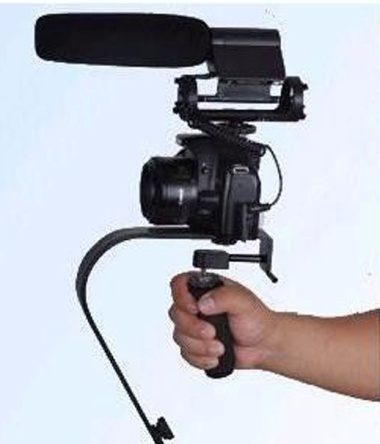
\includegraphics[width=.85\linewidth]{image1}
\captionof{figure}{ \label{fig:CCMP:2021:01}Bassin de traction}
\end{center}

\begin{center}
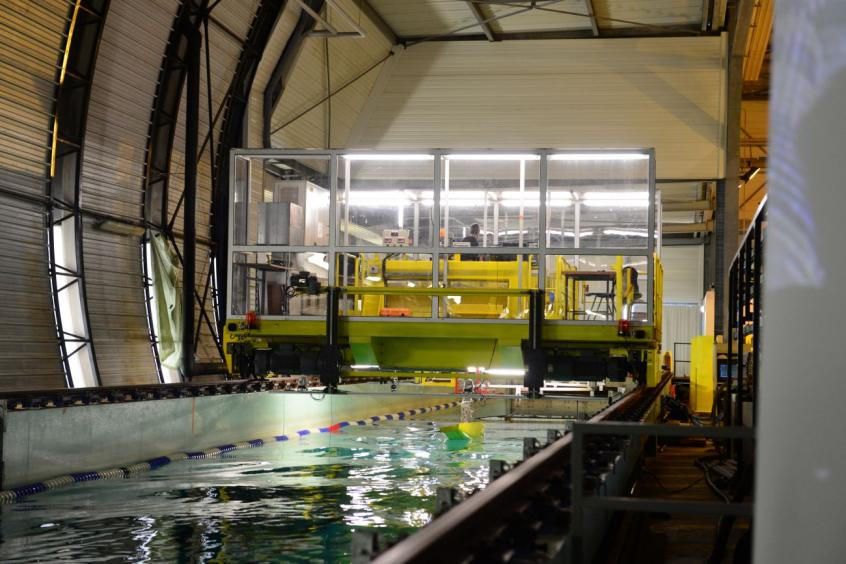
\includegraphics[width=.85\linewidth]{image2}
\captionof{figure}{ \label{fig:CCMP:2021:02}Chariot de traction}
\end{center}
\end{multicols}

Ce bassin, 2ème plus grand bassin de traction en France et le 1er au niveau académique, permet de mener un certain nombre d’expériences :
\begin{itemize}
	\item études de navires sur eau calme et sur houle ;
	\item tests de résistance à l'avancement de navires avec ou sans houle ;
	\item optimisations de carènes, tenue à la mer de navires ou structures flottantes ;
	\item tests de technologies en Energies Marines Renouvelables.
\end{itemize}
 
Il a par exemple servi aux tests menés sur la nouvelle hydrolienne développée par Alstom (Figure \ref{fig:CCMP:2021:03}).
L’industriel a utilisé une maquette de l’hydrolienne sur ce bassin de traction afin d’étudier son comportement pendant la phase de remorquage et, ainsi, vérifier jusqu’à quel état de mer elle pouvait être tractée.
L’analyse fonctionnelle globale de ce bassin est disponible en Annexe 2. Le diagramme des exigences est consultable en Annexe 4.
 
 \begin{figure}[!h]
\centering

\includegraphics[width=.45\linewidth]{image3}
\caption{ \label{fig:CCMP:2021:03} Maquette de l'Hydrolienne testée par Alstom }
\end{figure} 

\section{Étude de l'exigence 1.1.1 : « Durée de l'essai »}
\begin{obj}
Choisir un matériau pour la bande de roulement de chaque roue en contact avec le rail, afin de permettre des mesures correctes pendant une durée de mesure $\indice{t}{acq}$ donnée.
\end{obj}

\subsection{Détermination de l'accélération minimale}
Dans un premier temps, on va déterminer l'accélération minimale nécessaire pour que le chariot puisse se déplacer à une vitesse constante $V_m=\SI{8}{m.s^{-1}}$ pendant une durée d'acquisition $\indice{t}{acq}=\SI{10}{s}$.

\subsubsection*{Modélisation}
Lors d'un essai, le chariot \textbf{(3)} (voir Figure \ref{fig:CCMP:2021:05}) se déplace par rapport au sol \textbf{(0)} en translation rectiligne à une vitesse $V_3 (t)$ qui suit une loi de vitesse (Figure \ref{fig:CCMP:2021:04}) découpée en 3 phases :
\begin{itemize}
	\item première phase :	accélération $\gamma = \deriv{V_3(t)}{}$ constante ($\gamma >0$) jusqu'à atteindre la vitesse terminale souhaitée $V_3 (t)=V_m$;
	\item deuxième phase :	vitesse terminale conservée pendant la durée de l'acquisition $\indice{t}{acq}=T_2-T_1$ ;
	\item troisième phase :	décélération $-\gamma = \deriv{V_3(t)}{}$ constante ($\gamma >0$) jusqu'à l'arrêt complet.
\end{itemize}

Le profil de vitesse adopté est le suivant :
  
\begin{figure}[!h]
\centering
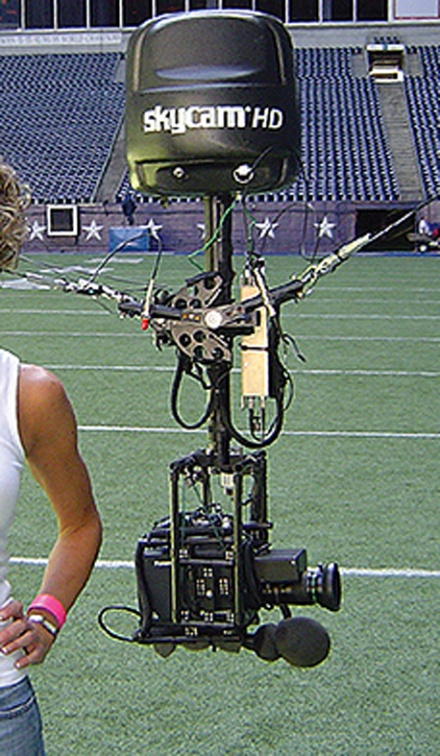
\includegraphics[width=.7\linewidth]{image4}
\caption{ \label{fig:CCMP:2021:04} Profil de vitesse souhaité du chariot}
\end{figure} 

À chaque essai, le chariot part d'une position initiale $X_0$ et termine sa course à une position finale $X_f$.
\subsubsection*{Données}
Pour rappel, la longueur complète du bassin est de \SI{140}{m}. Le chariot doit observer une distance de sécurité à chaque extrémité du bassin. Autrement dit on prendra $X_0=\SI{10}{m}$ et $X_f=\SI{130}{m}$.
La vitesse de déplacement du chariot par rapport au sol pendant la deuxième phase sera prise maximale et égale à $V_m=\SI{8}{m.s^{-1}}$. La durée de l'acquisition sera prise égale à $\indice{t}{acq}=\SI{10}{s}$.


% Q1
\question{\label{q:CCMP:2021:01}À partir de la Figure \ref{fig:CCMP:2021:04}, donner l'expression littérale du temps $T_1$ nécessaire pour avoir $\indice{t}{acq}=\SI{10}{s}$. En déduire l’expression littérale de l'accélération $\gamma$  de la première phase en fonction de $V_m$, $\indice{t}{acq}$,  $X_0$ et $X_f$. Faire l’application numérique.}
\ifprof
\begin{corrige}
On a :
\begin{itemize}
\item $X_0 = \dfrac{V_m T_1}{2}$
\item $\gamma = \dfrac{V_m}{T_1}$; 
\item $T_1 V_m + \indice{t}{acq}V_m = X_0 + X_f$ (aire sous le trapèze). 
\end{itemize}
En conséquences, $T_1   =\dfrac{X_0 + X_f -  \indice{t}{acq}V_m}{V_m}$ et 
$\gamma= \dfrac{V_m^2}{X_0 + X_f -  \indice{t}{acq}V_m}$

\textit{Applications numériques :}$\gamma = \dfrac{64}{140-80} \simeq \SI{1}{m.s^{-2}}$ et $T_1\simeq \SI{8}{s}$. 

\textit{Vérifications :} $X_0=\dfrac{1,0666\times 8}{2} =$ 
\end{corrige}
\else
\fi

\subsection{Dimensionnement de la motorisation}
Dans cette partie, on va dimensionner la motorisation en déterminant notamment le couple à fournir afin de satisfaire l’exigence 1.1.1.
\subsubsection{Modélisation}
Le chariot est composé (comme l'indique le Diagramme de Définition de Blocs en Annexe 5) de quatre roues motrices et de quatre roues libres en rotation. Pour des raisons de symétrie, on ne considère qu'une moitié du chariot. On fait alors l’hypothèse de problème plan, dans le plan $\left(G_3,\vx{0},\vy{0}, )\right)$. Il ne reste alors que deux roues motrices et deux roues libres en rotation (comme l’illustre le schéma cinématique complet en Annexe 6).

Pour les questions 2 à 9, et par souci de simplification, on fera l'étude à partir du schéma cinématique simplifié de la Figure \ref{fig:CCMP:2021:05} où seules les deux roues motrices ont été conservées.

Schéma de principe : 
\begin{figure}[!h]
\centering
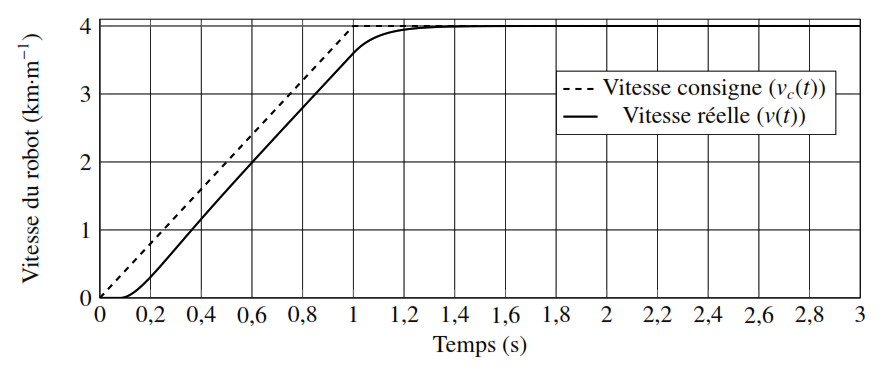
\includegraphics[width=.45\linewidth]{image5}
\caption{ \label{fig:CCMP:2021:05} Modélisation plane simplifiée du chariot (moteurs et réducteurs non représentés)}
\end{figure} 

Chaine de puissance :
\begin{figure}[!h]
\centering
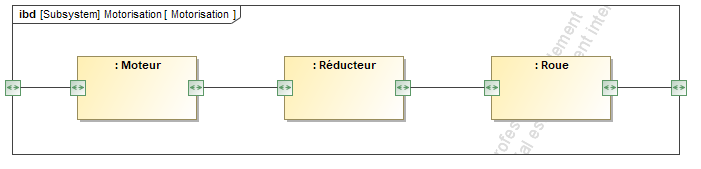
\includegraphics[width=.9\linewidth]{image6}
\caption{ \label{fig:CCMP:2021:06} Chaine de puissance de la motorisation pour une roue}
\end{figure} 
 



\subsubsection*{Données et notations}
\begin{itemize}
     \item La plateforme \textbf{(3)} a pour centre de gravité le point $G_3$ et pour masse $m_3$.
     \item Le mouvement de la plateforme sera défini par la vitesse $\vectv{G_3}{3}{0}=  V_3\vect{x_0}$ et par l'accélération $\vectv{G_3}{3}{0}=  \gamma \vect{x_0}$
     \item Le point $O_1$ est le centre d’inertie de la roue motrice avant \textbf{(1)}, le point $O_2$ est celui de la roue motrice arrière \textbf{(2)}. Chaque roue motrice possède une masse $m_R$ et un moment d'inertie $J_R$ par rapport à son axe de rotation dans son mouvement par rapport à \textbf{(3)}. Les roues sont équilibrées dynamiquement. Le rayon de chaque roue motrice est $R$.
     \item On définit les 2 grandeurs cinématiques suivantes : $\omega_m$ vitesse de rotation du rotor du moteur par rapport à \textbf{(3)} et $\omega_R$ vitesse de rotation des roues \textbf{(1)} et \textbf{(2)} par rapport à \textbf{(3)} (telle que $\vecto{1}{3}=\vecto{1}{3}=\omega_R \vz{0}$)****. Le moteur est alimenté en puissance électrique caractérisée par le courant $I_m$ parcourant le moteur et par la tension $U_m$ aux bornes de son induit.
     \item Au niveau de chaque roue, le réducteur (non représenté sur la Figure \ref{fig:CCMP:2021:05}) positionné entre le moteur et la roue motrice possède un rapport de réduction noté $k$ vérifiant $\omega_R= k \omega_m$.
\end{itemize}

\begin{multicols}{3}
\begin{itemize}
     \item $\vect{O_1 G_3} =-L\vx{0}+H\vy{0}$
     \item $\vect{O_2 G_3} =L\vx{0}+H\vy{0}$
     \item $H=\SI{1}{m}$
     \item $R=\SI{0,25}{m}$
     \item $L=\SI{2}{m}$
     \item $m_3=\SI{6000}{kg}$
     \item $m_R=\SI{200}{kg}$
     \item $J_R=\SI{20}{kg.m^2}$
     \item $k=1/25$
     \item $g=-g\vy{0}$ avec $g=\SI{10}{m.s^{-2}}$
\end{itemize} 
\end{multicols}

\subsubsection*{Hypothèses}
\begin{itemize}
    \item Les contacts entre les roues et le rail seront considérés avec frottement (le facteur de frottement est noté $f$ et on néglige la résistance au roulement), et on fait l'hypothèse de roulement sans glissement au niveau de ces contacts.
    \item Toutes les autres liaisons seront supposées parfaites. On supposera aussi que le réducteur est de rendement énergétique unitaire.
    \item Les actions mécaniques résistant à l'avancement et dues à l'action de l'air sur le chariot et à l'action de l'eau sur la maquette seront négligées par rapport aux effets dynamiques.
    \item Les masses et moments d’inertie des moteurs et des réducteurs seront négligés.
    \item Le sol du laboratoire \textbf{(0)} sera pris comme un référentiel galiléen de base $b_0=\left(\vx{0},\vy{0},\vz{0}\right)$.
\end{itemize}
\subsubsection*{Modélisation des actions mécaniques et notations retenues}
\begin{itemize}
    \item Pour toutes les actions mécaniques inconnues qu'il sera pertinent de définir, on utilisera la notation suivante (écriture avec problème plan) :
	$\torseurstat{T}{i}{j}=\torseurl{\vectf{i}{j}}{K}{K}$ $=\torseurcol{X_{ij}}{Y_{ij}}{-}{-}{-}{N_{ij}}{K,b_0}$

    \item Pour la motorisation des roues \textbf{(1)} et \textbf{(2)}, les actions respectives du rotor du moteur sur l’arbre d’entrée du réducteur seront modélisées par :
    $\torseurstat{T}{\text{mot}_1}{\text{red}_1}=\torseurl{\vect{0}}{C_m\vect{z_0}}{O_1} 
    \quad \quad
    \torseurstat{T}{\text{mot}_2}{\text{red}_2}=\torseurl{\vect{0}}{C_m\vect{z_0}}{O_2}$
    \item De la même manière, les actions respectives de l’arbre de sortie du réducteur sur la roue seront modélisées par :
    $\torseurstat{T}{\text{red}_1}{1}=\torseurl{\vect{0}}{C_R\vect{z_0}}{O_1} 
    \quad \quad
    \torseurstat{T}{\text{red}_2}{2}=\torseurl{\vect{0}}{C_R\vect{z_0}}{O_2}$
    \item Les réducteurs étant considérés parfaits, on admettra que :	 $C_m = k C_R$.
\end{itemize}


On isole l'ensemble du chariot $\Sigma=\textbf{(1)}\cup \textbf{(2)}\cup \textbf{(3)}\cup (\text{\textbf{moto-réducteurs}})$.


% Q2
\question{\label{q:CCMP:2021:02}Exprimer $V_3$ en fonction de $\omega_R$. Déterminer l'énergie cinétique $\ec{\Sigma}{0}$ de l'ensemble isolé par rapport à \textbf{(0)} (on écrira le résultat en fonction de $V_3$). En déduire la masse équivalente $\indice{M}{eq}$, ramenée sur \textbf{(3)}, de l'ensemble isolé, telle que $\ec{\Sigma}{0}=\dfrac{1}{2} \indice{M}{eq} V_3^2$.}
\ifprof
\begin{corrige}
\end{corrige}
\else
\fi


% Q3
\question{\label{q:CCMP:2021:03} Lister l'ensemble des puissances galiléennes des actions mécaniques extérieures, et donner leur expression en fonction de $V_3$ et des paramètres du modèle. Reproduire la démarche avec la puissance des actions mécaniques intérieures.}
\ifprof
\begin{corrige}
\end{corrige}
\else
\fi

% Q4
\question{\label{q:CCMP:2021:4}Appliquer le Théorème de l'Énergie Cinétique (Énergie Puissance) pour déterminer l'expression du couple moteur $C_m$ au niveau de chaque moteur permettant d'assurer l’accélération $\gamma$ nécessaire.}
\ifprof
\begin{corrige}
\end{corrige}
\else
\fi


\subsection{Détermination du facteur de frottement minimal}
Afin d’éviter un phénomène de glissement entre les roues motrices et le rail au moment où l’accélération est maximale (phase 1, Figure \ref{fig:CCMP:2021:04}), il est nécessaire de déterminer le facteur de frottement minimal entre le rail et les roues. On pourra ainsi valider l’hypothèse de roulement sans glissement.

% Q5
\question{\label{q:CCMP:2021:5}Donner l'expression du moment dynamique de la roue avant \textbf{(1)} au point $O_1$ dans son mouvement par rapport au sol \textbf{(0)} en fonction de $\deriv{\omega_R (t)}{}$. Réaliser l'inventaire des actions mécaniques extérieures agissant sur \textbf{(1)} (donner l'expression de chaque torseur).}
\ifprof
\begin{corrige}
\end{corrige}
\else
\fi


% Q6
\question{\label{q:CCMP:2021:} On isole la roue avant \textbf{(1)}. Écrire le théorème du moment
dynamique appliqué à la roue \textbf{(1)} au point $O_1$ projeté sur $\vz{0}$, puis en déduire
l'expression littérale de la composante $X_{01}$ (de l'action du sol \textbf{(0)} sur la roue \textbf{(1)})
en fonction uniquement de l'accélération $\gamma$ et des masses. Donner alors, sans faire le calcul,
l'expression littérale de la composante $X_{02}$ de l'action du sol \textbf{(0)} sur la roue \textbf{(2)}.}
\ifprof
\begin{corrige}
\end{corrige}
\else
\fi


% Q7
\question{\label{q:CCMP:2021:7}On isole l'ensemble du chariot $\Sigma=\textbf{(1)}\cup \textbf{(2)}\cup \textbf{(3)}\cup (\text{\textbf{moto-réducteurs}})$. Proposer le théorème utilisé (T.R.D. ou T.M.D., la projection, éventuellement le point) permettant de déterminer la composante $Y_{01}$. Donner l’expression de la composante du torseur dynamique correspondant en fonction de $\gamma$, des différentes masses et/ou inerties ainsi que des grandeurs géométriques.}
\ifprof
\begin{corrige}
\end{corrige}
\else
\fi

% Q8
\question{\label{q:CCMP:2021:8}Proposer uniquement la démarche (isolement(s), inventaire des actions mécaniques, théorème(s) utilisé(s)) permettant ensuite de déterminer la composante $Y_{02}$ de l'action du sol \textbf{(0)} sur la roue \textbf{(2)}.}
\ifprof
\begin{corrige}
\end{corrige}
\else
\fi

Une application numérique a permis de déterminer, sous les hypothèses fournies précédemment, la valeur minimale pour assurer le non-glissement du facteur de frottement noté $f_1$ au niveau de la roue motrice avant \textbf{(1)} puis celle du facteur de frottement noté $f_2$ au niveau de la roue motrice arrière \textbf{(2)} : $f_1=0,177$ et $f_2=0,146$.

% Q9
\question{\label{q:CCMP:2021:9}Dans un premier temps, en se basant sur les lois de Coulomb, indiquer la démarche qui a été mise en œuvre pour déterminer les valeurs minimales de $f_1$ et $f_2$.}
\ifprof
\begin{corrige}
\end{corrige}
\else
\fi

En réalité, le chariot ne possède pas uniquement quatre roues motrices (deux de chaque côté), mais deux bogies constitués chacun de deux roues motrices et de deux roues libres en rotation (Annexe 6). La présence d'une roue libre en rotation sur chaque côté d'un bogie permet de soulager environ de moitié l'effort normal sur chaque roue motrice, tandis que l'effort tangentiel sur chaque roue motrice reste identique.
Le rail sur lequel les roues roulent sans glisser est en acier. On souhaite utiliser le même matériau pour toutes les roues (avant comme arrière, motrices comme libres).
On adoptera un coefficient de sécurité $s=2$ afin de garantir la pertinence des résultats en tenant compte des hypothèses simplificatrices adoptées lors de la modélisation.

% Q10
\question{\label{q:CCMP:2021:10}À partir des indications fournies, proposer une valeur du facteur de frottement à retenir et justifier. Enfin, à partir du Tableau \ref{tab:CCMP:2021:01} ci-dessous, proposer un choix de bandage (matériau de chaque roue) qui permette d’éviter le glissement en phase d’accélération, pour ainsi respecter l'exigence 1.1.1.}
\ifprof
\begin{corrige}
\end{corrige}
\else
\fi


\begin{table}[!h]
\centering
\begin{tabular}{lll}
\hline
\textbf{Matériau 1} & \textbf{Matériau 2} & \textbf{Facteur de frottement sec} \\ 
\hline
Acier	& Téflon & 0,05 \\
Acier	& Acier (sec) & 0,2\\
Acier	& PVC & 0,5\\
Acier	& Caoutchouc & 1 à 4\\
\hline
\end{tabular}
\caption{ \label{tab:CCMP:2021:01} Facteur de frottement en fonction du couple de matériaux - contact sec}
\end{table} 

\section{Étude de l'exigence 3 : « Acquérir les données »}
\begin{obj}
Déterminer l'ensemble des composantes du torseur des actions mécaniques de l'eau agissant sur la maquette en déplacement à vitesse stabilisée.
\end{obj}
\subsection{Principe de la mesure de l’action de l’eau sur la maquette}
La maquette de bateau à étudier et le mât métallique de support forment l’ensemble \textbf{\textbf{(5)}}. Cet ensemble est lié à la plateforme \textbf{(3)} par l’intermédiaire du solide \textbf{(4)} et de 6 barres 
$(B_1)$, $(B_2)$, …, $(B_6)$ dotées chacune d’un capteur dynamométrique (voir Figure \ref{fig:CCMP:2021:07} ci-dessous ainsi que les photos en Annexe 7).
 
\begin{figure}[!h]
\centering

\includegraphics[width=.45\linewidth]{image7}
\caption{ \label{fig:CCMP:2021:07} Schéma cinématique 3D du dispositif de mesure}
\end{figure} 

\subsubsection*{Données et hypothèses}
 \begin{itemize}
 \item $OA=OC=OD=a$
 \item $OB=d$
 \item $\vect{OL}=-e.\vx{0}+f.\vz{0}$
 \item $\vect{LG_5}=-\lambda (t) \vy{0}$
 \item Toutes les barres $(B_i)$ ont la même longueur a, et on considèrera leur masse négligeable.
 \item $m_4$ est la masse du solide \textbf{(4)}, de centre d’inertie $O$.
\end{itemize} 

Les liaisons représentées en A et en C sont constituées chacune de 2 liaisons sphériques concentriques $\mathcal{L}_{B_1/4}$ et $\mathcal{L}_{B_5/4}$ sphériques en $A$, et $\mathcal{L}_{B_2/4}$ et $\mathcal{L}_{B_6/4}$ en $C$).
Dans toute la partie 3, on considèrera la plateforme \textbf{(3)} immobile.
La fonction principale de ce dispositif est de mesurer les actions mécaniques qu’exerce l’eau sur la maquette de bateau. On cherche donc à mesurer à tout instant $\torseurstat{T}{\text{eau}}{5}$ au point $G_5$, centre d’inertie de l’ensemble \textbf{(5)}.
Étude de la liaison entre l’ensemble \textbf{(5)} et le solide \textbf{(4)}
La maquette est en liaison encastrement avec un mât métallique (ensemble \textbf{(5)}), lui-même en liaison avec le solide \textbf{(4)} par l’intermédiaire de 7 liaisons sphère/plan (Figure \ref{fig:CCMP:2021:08}).


\begin{figure}[!h]
\centering
    \begin{subfigure}[b]{.3\textwidth}
    \centering
    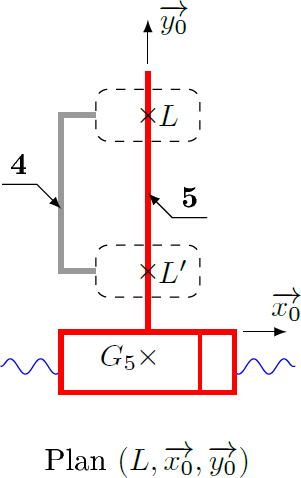
\includegraphics[width=.9\linewidth]{image8_a}
    \caption{Figure \ref{fig:CCMP:2021:08}a \label{fig:CCMP:2021:08:a}}
    \end{subfigure}
    \hfill
    \begin{subfigure}[b]{.3\textwidth}
    \centering
    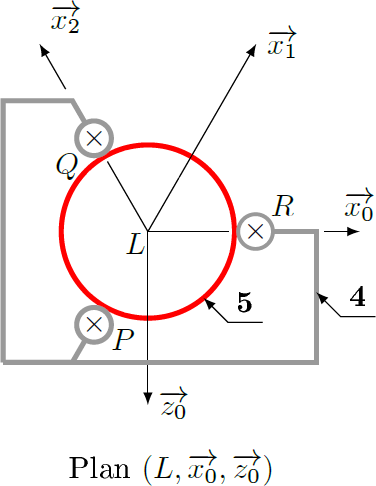
\includegraphics[width=.9\linewidth]{image8_b}
    \caption{Figure \ref{fig:CCMP:2021:08}b \label{fig:CCMP:2021:08:b}}
    \end{subfigure}
    \hfill
    \begin{subfigure}[b]{.3\textwidth}
    \centering
    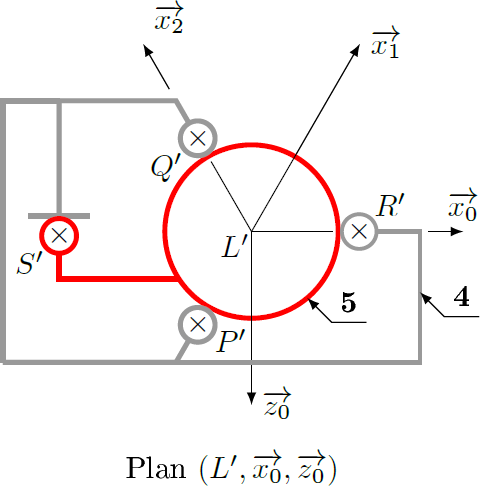
\includegraphics[width=.9\linewidth]{image8_c}
    \caption{Figure \ref{fig:CCMP:2021:08}c \label{fig:CCMP:2021:08:c}}
    \end{subfigure}
%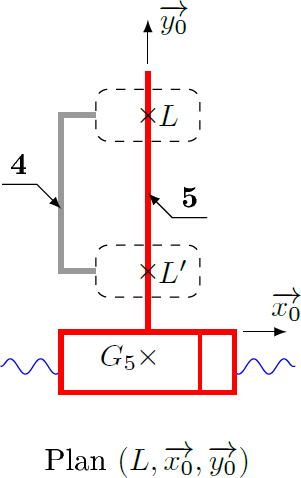
\includegraphics[width=.45\linewidth]{image8_a}
\caption{ \label{fig:CCMP:2021:08} Modélisation de la liaison entre \textbf{(4)} et \textbf{(5)}}
\end{figure}


\subsubsection*{Données}
\begin{itemize}
\item $LP=L'P' = LQ  = L'Q' = LR = L'R' = r_5$,
\item $\vect{S'L'} = d_5 \vx{0}$, $\vect{LL'} = -h_5 \vy{0}$, $\vect{LG_5}=-\lambda(t) \vy{0}$
\item $\alpha  =(\vx{0},\vx{1})=(\vx{1},\vx{2})=\dfrac{\pi}{3}$
$\left\{ \mathcal{T}^R \left(4\to 5 \right) \right\} = \torseurcol{X_R}{0}{0}{0}{0}{0}{R,b_0}$
$\left\{ \mathcal{T}^P \left(4\to 5 \right) \right\} = \torseurcol{X_P}{0}{0}{0}{0}{0}{P,b_1}$
$\left\{ \mathcal{T}^Q \left(4\to 5 \right) \right\} = \torseurcol{X_Q}{0}{0}{0}{0}{0}{Q,b_2}$.
\end{itemize}
\subsubsection*{Notations}
\begin{itemize}
    \item $\left\{ \mathcal{T}^1 \left(4\to 5 \right) \right\}$ : torseur des actions mécaniques transmissibles par la liaison équivalente aux 3 liaisons représentées sur la Figure \ref{fig:CCMP:2021:08:b}.
    \item $\left\{ \mathcal{T}^2 \left(4\to 5 \right) \right\}$ : torseur des actions mécaniques transmissibles par la liaison équivalente aux 4 liaisons représentées sur la Figure \ref{fig:CCMP:2021:08:c}.
    \item $\left\{ \mathcal{T} \left(4\to 5 \right) \right\}$ : torseur des actions mécaniques transmissibles par la liaison équivalente entre \textbf{(4)} et \textbf{(5)}.
\end{itemize}
Pour les questions \ref{q:CCMP:2021:11} et \ref{q:CCMP:2021:12}, on cherchera à simplifier les torseurs suivants en remplaçant les termes nuls par des 0 :
$\left\{ \mathcal{T}^1 \left(4\to 5 \right) \right\} = \torseurcol{X_1}{Y_1}{Z_1}{L_1}{M_1}{N_1}{L,b_0}$
$\left\{ \mathcal{T}^2 \left(4\to 5 \right) \right\} = \torseurcol{X_2}{Y_2}{Z_2}{L_2}{M_2}{N_2}{L',b_0}$
$\left\{ \mathcal{T} \left(4\to 5 \right) \right\} = \torseurcol{X_{45}}{Y_{45}}{Z_{45}}{L_{45}}{M_{45}}{N_{45}}{Q,b_2}$ 

% Q11
\question{\label{q:CCMP:2021:11}Préciser votre démarche puis donner l'écriture simplifiée du torseur $\left\{ \mathcal{T}^1 \left(4\to 5 \right) \right\}$ au point $L$ puis donner le nom et la (les) caractéristique(s) géométrique(s) de cette liaison. Donner également l'écriture simplifiée du torseur $\left\{ \mathcal{T}^2 \left(4\to 5 \right) \right\}$ au point $L'$. Les torseurs seront exprimés dans la base $b_0=\left(\vx{0},\vy{0},\vz{0} \right)$.}
\ifprof
\begin{corrige}
\end{corrige}
\else
\fi

% Q12
\question{\label{q:CCMP:2021:12}Donner l'écriture simplifiée de $\left\{ \mathcal{T}\left(4\to 5 \right) \right\}$, torseur des actions mécaniques transmissibles par la liaison équivalente entre \textbf{(4)} et \textbf{(5)} en $L$ (également exprimé dans la base $b_0$). Donner le nom et la (les) caractéristique(s) géométrique(s) de cette liaison. Expliquer pourquoi le concepteur a choisi une telle liaison plutôt qu’une liaison encastrement entre l’ensemble \textbf{(5)} et le solide \textbf{(4)}.}
\ifprof
\begin{corrige}
\end{corrige}
\else
\fi

\subsection{Réglage de la ligne de flottaison}
Dans un souci de polyvalence du banc de mesure, il est nécessaire de pouvoir régler la position de la ligne de flottaison (exigence 3.2.1). De plus, il est important de compenser la présence du dispositif de mesure (exigence 3.2.2), c'est à dire d'annuler l'influence du poids du mât vertical. Un système de poulie avec contrepoids a donc été ajouté pour satisfaire conjointement ces deux exigences (Figure \ref{fig:CCMP:2021:09}).

On note $m_5$ la masse de l'ensemble \textbf{(5)}, considéré homogène et $m_7$ la masse du contrepoids \textbf{(7)}. Connaissant la géométrie de la coque (simplifiée sur la Figure \ref{fig:CCMP:2021:09}), on souhaite pouvoir régler la hauteur immergée $h_i$.

\begin{figure}[!h]
\centering
    \begin{subfigure}[b]{.3\textwidth}
    \centering
    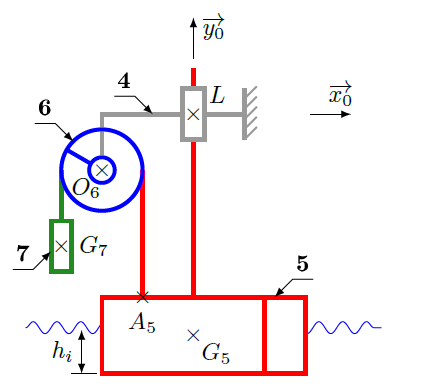
\includegraphics[width=\linewidth]{image9_a}
    \caption{\label{fig:CCMP:2021:09:a}Vue d’ensemble }
    \end{subfigure}
    \begin{subfigure}[b]{.3\textwidth}
    \centering
    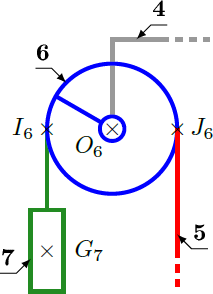
\includegraphics[width=.8\linewidth]{image9_b}
    \caption{\label{fig:CCMP:2021:09:b} Poulie (6)}
    \end{subfigure}
    \begin{subfigure}[b]{.3\textwidth}
    \centering
    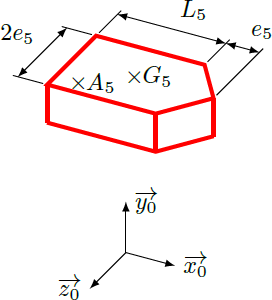
\includegraphics[width=\linewidth]{image9_c}
    \caption{\label{fig:CCMP:2021:09:c} Modèle du bateau}
    \end{subfigure}
\caption{ \label{fig:CCMP:2021:09}Système de réglage de la ligne de flottaison}
\end{figure}

 
\subsubsection*{Hypothèses}
\begin{itemize}
\item On considère le système à l’arrêt. Ainsi, le solide \textbf{(4)} est immobile par rapport au sol.
\item Pour les questions \ref{q:CCMP:2021:13} à \ref{q:CCMP:2021:15}, on considère que le bassin ne génère pas de houle. On admettra alors que la poussée d’Archimède est la seule action mécanique exercée par l’eau sur la maquette. Cette action mécanique sera modélisée par un glisseur passant par $G_5$, de direction verticale, dirigée du bas vers le haut et de norme égale au poids du volume d’eau déplacé (volume correspondant au volume de la partie immergée de la maquette).
\item Les masses du câble et de la poulie sont négligées. Le câble ne glisse pas sur la poulie, et les brins tendus seront considérés comme inextensibles dans le cadre d’une étude statique. Le câble est lié à la maquette en $A_5$.
\item On admettra que le brin tendu lié à la maquette exerce sur la poulie l’action mécanique suivante :
$\left\{ \mathcal{T} \left(5\to 6 \right) \right\} = \torseurl{F_{56}\vy{0}}{\vect{0}}{J_6}$.
\end{itemize}


\subsubsection*{Données}
\begin{itemize}
    \item $\vect{I_6 G_7}  = -l_6 \vect{y_0}$;
    \item $\vect{G_5 A_5} = -a_5\vx{0}+b_5 \vy{0}+c_5 \vz{0}$;
    \item $\vect{A_5 J_6 } = l_6 \vy{0}$;
    \item $R_6$ : rayon de la poulie \textbf{(6)};
    \item $\rho$ : masse volumique de l’eau.
\end{itemize} 


% Q13
\question{\label{q:CCMP:2021:13}En appliquant le Principe Fondamental de la Statique à l’ensemble \textbf{\{6+7\}}, exprimer $F_{56}$ en fonction de $m_7$,  $g$ et des paramètres géométriques nécessaires. Préciser la ou les équations utilisées.}
\ifprof
\begin{corrige}
\end{corrige}
\else
\fi

% Q14
\question{\label{q:CCMP:2021:14}Exprimer le torseur modélisant l’action de la poussée d’Archimède sur la maquette $\torseurstat{T}{\text{eau}}{5}$, au point $G_5$, en fonction de $L_5$, $e_5$, $h_i$, $\rho$ et $g$. En appliquant le Principe Fondamental de la Statique à \textbf{(5)}, en déduire la hauteur de maquette immergée $h_i$ en fonction de $m_5$, $m_7$, $\rho$, $e_5$ et $L_5$.}
\ifprof
\begin{corrige}
\end{corrige}
\else
\fi

% Q15
\question{\label{q:CCMP:2021:15}Montrer que ce dispositif permet à lui seul de satisfaire les exigences 3.2.1 et 3.2.2. L’emplacement du point d’ancrage du câble du contrepoids sur la maquette a-t-il une influence sur la hauteur immergée ?}
\ifprof
\begin{corrige}
\end{corrige}
\else
\fi

\subsection{Détermination du torseur des actions mécaniques de l’eau sur la maquette}

\begin{obj}L’objectif de cette étude est de trouver une relation entre les mesures des 6 capteurs dynamométriques et le torseur des actions mécaniques de l’eau sur la maquette (Figure \ref{fig:CCMP:2021:07} ou Annexe 7 et Figure \ref{fig:CCMP:2021:09}), lorsque le bassin génère une houle.
\end{obj}


\subsubsection*{Hypothèses}
\begin{itemize}
    \item On considèrera dans la partie 3.4 que la plateforme \textbf{(3)} est toujours à l’arrêt. Du fait de la géométrie du mécanisme, \textbf{(4)} est donc immobile par rapport à \textbf{(3)}.
    \item On rappelle que les masses des barres \textbf{(Bi)} seront négligées dans cette étude.
    \item Le bassin génère maintenant une houle, donc $\lambda(t)$ varie au cours du temps. Conformément au paramétrage de la partie 3.1, on définit alors : ($\vectg{G_5}{5}{4}=\gamma_5 \vy{0}$ avec $\gamma_5=- \dderiv{\lambda(t)}{}$.
    \item La modélisation de $\torseurstat{T}{\text{eau}}{5}$ est maintenant définie par :
    $\torseurstat{T}{\text{eau}}{5} =  \torseurcol{X_e}{Y_e}{Z_e}{L_e}{M_e}{N_e}{G_5,b_0}$ 
\end{itemize}


% Q16
\question{\label{q:CCMP:2021:}Sur la base de la Figure \ref{fig:CCMP:2021:07}, on considère le système constitué des solides \textbf{(3)}, \textbf{(4)} et des 6 barres \textbf{(Bi)}. Déterminer le degré d’hyperstatisme du modèle proposé. Que peut-on en déduire ?}
\ifprof
\begin{corrige}
\end{corrige}
\else
\fi

En considérant que les distances $a_5$ et $c_5$ sont très petites, une étude dynamique préliminaire a permis d’établir que l’action du câble sur la maquette s’écrit en $G_5$ : $\torseurstat{T}{6}{5}= \torseurl{m_7 \left(g-\gamma_5\right) \vy{0}}{\vect{0}}{G_5}$


% Q17
\question{\label{q:CCMP:2021:17}En tenant compte des hypothèses précédentes, déterminer le torseur $\torseurstat{T}{4}{5}$ (exprimé au point $L$) des actions mécaniques transmises par la liaison glissière entre \textbf{(4)} sur \textbf{(5)} en fonction de $X_e$, $Y_e$, ..., $N_e$ et des différents paramètres géométriques. On exprimera le résultat dans $b_0$.}
\ifprof
\begin{corrige}
\end{corrige}
\else
\fi

% Q18
\question{\label{q:CCMP:2021:18}Sachant que les coordonnées de $\torseurstat{T}{4}{5}$ seront mesurées par les 6 capteurs dynamométriques de la balance, indiquer s’il est possible de mesurer $Y_e$ avec ce dispositif. Justifier.}
\ifprof
\begin{corrige}
\end{corrige}
\else
\fi

On note $F_1$, $F_2$, …, $F_6$ les valeurs algébriques mesurées par les 6 capteurs  $\left(c_1, c_2, ..., c_6\right)$ telles que, pour une barre \textbf{(Bi)} de direction $\vect{u_i}$ :  $\torseurstat{T}{B_i}{4}=\torseurl{F_i \vect{u_i}}{\vect{0}}{M_i}$  avec le point $M_i$ à choisir parmi les points $A$, $B$, $C$ et $D$.

% Q19
\question{\label{q:CCMP:2021:19}Montrer que l'action mécanique de la barre \textbf{(B1)} sur \textbf{(4)} est un glisseur et préciser son axe.}
\ifprof
\begin{corrige}
\end{corrige}
\else
\fi


% Q20
\question{\label{q:CCMP:2021:20}Exprimer en fonction des $F_i$ la forme des torseurs des actions mécaniques suivantes dans la base $b_0$ : 
$\torseurstat{T}{B_1}{4}$, $\torseurstat{T}{B_2}{4}$, $\torseurstat{T}{B_3}{4}$, 
$\torseurstat{T}{B_4}{4}$, $\torseurstat{T}{B_5}{4}$ et $\torseurstat{T}{B_6}{4}$.}
\ifprof
\begin{corrige}
\end{corrige}
\else
\fi


Quels que soient les résultats obtenus précédemment, on admettra pour la suite :
$\torseurstat{T}{5}{4}=\torseurcol{X_e}{0}{Z_e}{L_e-\lambda(t)Z_e}{M_e + eZ_e}{M_e+eZ_e + fX_e}{N_e + \lambda(t)X_e}{O,b_0}$

% Q21
\question{\label{q:CCMP:2021:21}Déterminer les expressions de $X_e$, $Z_e$, $L_e$, $M_e$ et $N_e$ en fonction de $F_1$, $F_2$,…, $F_6$ et des diverses grandeurs géométriques.}
\ifprof
\begin{corrige}
\end{corrige}
\else
\fi

% Q22
\question{\label{q:CCMP:2021:22}Au vu des expressions précédentes, quelle(s) grandeur(s) est-il nécessaire de connaitre sur le système pour obtenir à tout instant une mesure de $X_e$, $Z_e$, $L_e$, $M_e$ et $N_e$ ? Proposer un dispositif permettant de connaitre cette (ces) grandeur(s) en temps réel.}
\ifprof
\begin{corrige}
\end{corrige}
\else
\fi

\section{\label{s:CCMP:2021:04}Étude de l'exigence 1.2 : « Garantir un dÉplacement du chariot à vitesse constante »}
\begin{obj}
Modéliser l'asservissement en vitesse du chariot de traction puis régler les paramètres du correcteur afin de satisfaire tous les critères de l'exigence 1.2 du cahier des charges.
\end{obj}

Dans toute la partie \ref{s:CCMP:2021:04}, on notera $F$ la transformée de Laplace de la fonction $f$ :	$F(p)=\mathcal{L}\left[f(t)\right]$
\subsection{Modélisation de l'asservissement en vitesse}

\subsubsection*{Principe de fonctionnement et schéma-blocs}

On étudie l'asservissement en vitesse du chariot de traction dont le schéma-blocs est donné en Figure \ref{fig:CCMP:2021:10}.

\begin{itemize}
\item Un adaptateur de gain $K_1$ permet de fournir l'image $U_C (p)$ de la consigne de vitesse $V_C (p)$.
\item Un capteur de vitesse en rotation de gain $K_{11}$ renvoie une tension $\indice{U}{mes}(p)$ proportionnelle à la vitesse de rotation $\indice{\Omega}{mes} (p)$ de son axe. Par ailleurs, une roue libre en rotation de gain $K_9$ associée à un réducteur de vitesse épicycloïdal de gain $K_{10}$ permettent de transformer la vitesse du chariot $V(p)$ en vitesse de rotation $\indice{\Omega}{mes} (p)$ de l'axe du capteur de vitesse de rotation.
\item L'écart $\varepsilon_U (p)$ entre $U_C (p)$ et $\indice{U}{mes} (p)$ est ensuite corrigé par un correcteur de fonction de transfert $C(p)$ afin de piloter un variateur de gain $K_2$.
\item La tension de commande $U_m (p)$ du moteur va induire la vitesse angulaire $\Omega_m (p)$ de l'axe moteur.
\item Un réducteur de vitesse de gain $K_7$ puis le système roue-rail de gain $K_8$ transforment le mouvement pour obtenir une vitesse $V(p)$ de translation du chariot.
\item On notera $\indice{F}{res} (p)$ la force de l'eau sur la maquette en mouvement. $\indice{C}{res} (p)$ représente le couple équivalent à $\indice{F}{res} (p)$ ramené sur l'axe moteur.
\end{itemize}
On rappelle qu'il y a roulement sans glissement entre la roue libre en rotation et le rail, ainsi qu’entre la roue motrice et le rail.
 
\begin{figure}[!h]
\centering
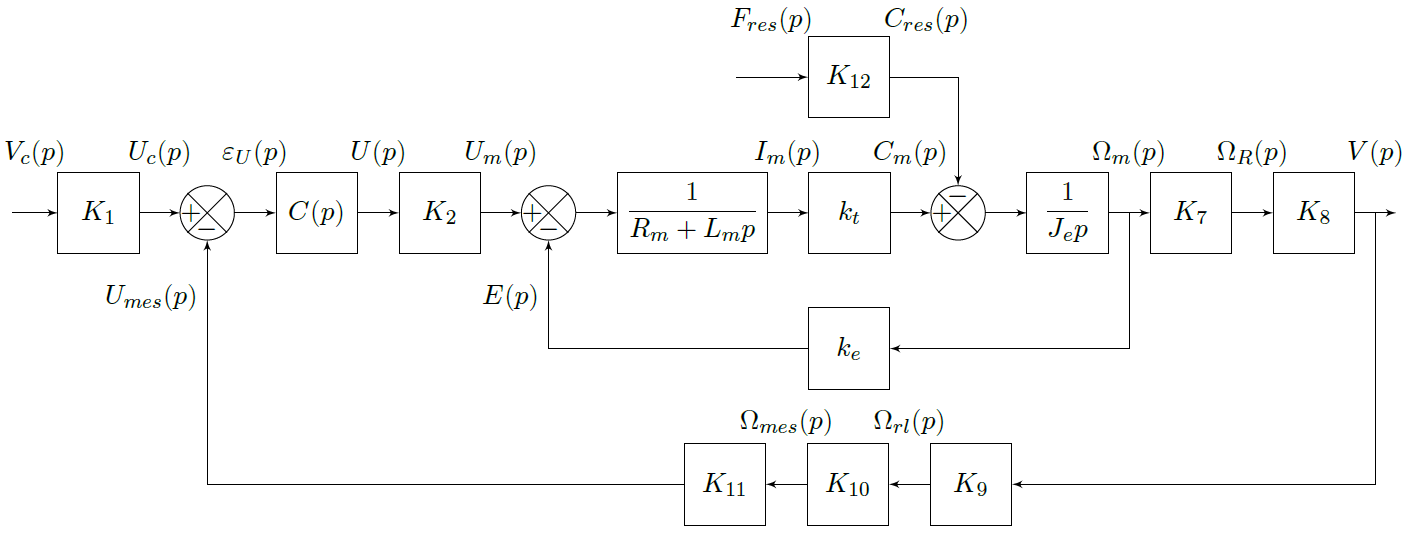
\includegraphics[width=\linewidth]{image10}
\caption{ \label{fig:CCMP:2021:10} Schéma-blocs de l'asservissement en vitesse du chariot}
\end{figure} 

\subsubsection*{Données générales}
 
 \begin{itemize}
\item Rayon de la roue motrice :	$R=\SI{0,25}{m}$
\item Rayon de la roue libre en rotation : $r=\SI{0,15}{m}$
\item Capteur de vitesse en rotation : $K_{11}=\SI{60}{V.s.rad^{-1}}$
\item Autres données : $K_2=1$ et $K_7=\mu=\dfrac{1}{25}$, $K_{10}=\dfrac{1}{2,5}$	$K_{12}=R\mu$.
 \end{itemize}
 
On souhaite compléter la modélisation de l'asservissement à partir du principe de fonctionnement fourni et des données générales.

% Q23
\question{\label{q:CCMP:2021:}Indiquer les expressions littérales des gains $K_8$ et $K_9$. Déterminer ensuite $K_1$ en fonction des autres gains $K_i$ permettant d’obtenir un écart $\varepsilon_U (p)$ nul lorsque la sortie $V(p)$ est égale à la consigne $V_c (p)$ (vous préciserez les unités de chacun des gains demandés).}
\ifprof
\begin{corrige}
\begin{itemize}
\item La vitesse du chariot est obtenue grâce à la mise en rotation de la roue motrice de rayon $R$ et il a été vu que$v(t)=-R\omega_r(t)$. De plus $V(p)=K_8\Omega_R(p)$. On a donc et $K_8 = -R$ et $K_8 = -\SI{0,25}{m}$.
\item De même en passant par la roue libre, $V(p)=r \Omega_{rl}(p)$ et $K_9 = -\dfrac{1}{r} = -\SI{6,67}{m^{-1}}$.
\item On a $\varepsilon_U(p)=V_C(p)K_1 - V(p) K_{11}K_{10}K_9$. Pour avoir un écart nul lorsque $V(p)=V_C(p)$, on a nécessairement $K_1 = K_{11}K_{10}K_9$. On a donc  $K_1 = 60\times \dfrac{1}{2,5}\times \dfrac{-1}{0,15}=  - \SI{160}{V.s.rad^{-1} m^{-1}}$.
\end{itemize}
\end{corrige}
\else
\fi


\subsection{Influence de la perturbation sur la réponse}
À partir de la modélisation initiale, on peut établir le schéma-blocs à retour unitaire de la Figure \ref{fig:CCMP:2021:11}. Sur ce schéma-blocs, on notera que la perturbation a été décalée en amont du moteur.
 

\begin{figure}[!h]
\centering
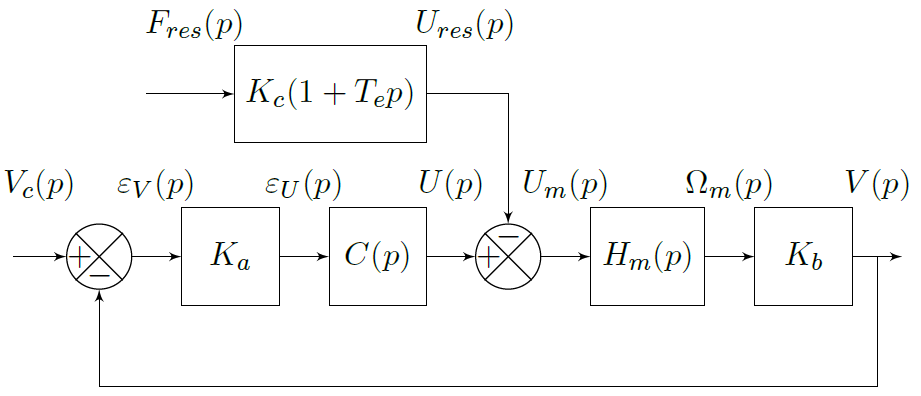
\includegraphics[width=.7\linewidth]{image11}
\caption{ \label{fig:CCMP:2021:11} Schéma-blocs simplifié de l'asservissement}
\end{figure}  
 
Avec :
\begin{itemize}
\item $K_a=\SI{1000}{V.s.m^{-1}}$
\item $K_b=\SI{0,01}{m}$
\item $K_c=\SI{0,1}{V.N^{-1}}$ avec $H_m (p)= \dfrac{K_m}{\left(1+T_e p\right) \left(1+T_m.p\right) }$
où $K_m=\SI{2}{rad.s^{-1}.V^{-1}}$ et $T_m=\SI{5}{s}$ et $T_e=\SI{0,5}{s}$.
\end{itemize}	
 

On fera dans un premier temps le choix d'un correcteur proportionnel : $C(p)=C$.
On notera $V(p)=V_1 (p)-V_2 (p)$ avec $V_1 (p)= H_1 (p) V_C (p)$ et $V_2 (p)=H_2 (p) \indice{F}{res}(p)$. On précise que :
\begin{itemize}
    \item $v_1 (t)$ est la réponse du système à la seule consigne et on note : $V_1 (p)=\mathcal{L}\left[v_1 (t)\right] $;
    \item $v_2 (t)$ est la réponse du système à la seule perturbation et on note : $V_2 (p)=\mathcal{L}\left[v_1 (t)\right]$.
\end{itemize}
On soumet le système à un échelon de consigne d'amplitude $V_0$ et à un échelon de perturbation d'amplitude $F_0$. Par linéarité, la réponse en régime permanent s'écrit comme suit :
$\lim\limits_{t\to \infty} = v_1 - v_2$ où $v_1=\lim\limits_{t\to \infty}v_1(t)$ et $v_2=\lim\limits_{t\to \infty}v_2(t)$.

Par souci de simplification, on notera également $\indice{K}{BO}=CK_a K_b K_m$.

% Q24
\question{\label{q:CCMP:2021:}Déterminer l'expression littérale des fonctions de transfert $H_1(p)$ et $H_2 (p)$ (la forme canonique n'est pas demandée). En déduire les expressions des réponses $v_1$ et $v_2$ en fonction de $V_0$, $F_0$, $\indice{K}{BO}$, $K_m$, $K_c$ et $K_b$.}
\ifprof
\begin{corrige}
Par lecture directe : $V(p)=U_m(p)H_m(p)K_b$ $=\left(\varepsilon_V(p) K_a C(p) - \indice{F}{res}(p)K_c\left(1+T_e p\right)\right) H_m(p)K_b$.
On a donc $V(p)=\left(\left(V_c(p) - V(p) \right) K_a C(p) - \indice{F}{res}(p)K_c\left(1+T_e p\right)\right) H_m(p)K_b$ et $V(p)=K_a C(p)H_m(p)K_bV_c(p) - H_m(p)K_bK_a C(p) V(p)  - \indice{F}{res}(p)K_c\left(1+T_e p\right)H_m(p)K_b$
Soit : 
$V(p)\left(1+ H_m(p)K_bK_a C(p)\right)  =K_a C(p)H_m(p)K_bV_c(p) - \indice{F}{res}(p)K_c\left(1+T_e p\right)H_m(p)K_b$ et 
$V(p) =\dfrac{K_a C(p)H_m(p)K_b}{1+ H_m(p)K_bK_a C(p)}V_c(p) -\dfrac{K_c\left(1+T_e p\right)H_m(p)K_b}{1+ H_m(p)K_bK_a C(p)} \indice{F}{res}(p)$.

Par ailleurs : 

$v_1=\lim\limits_{t\to \infty}v_1(t)=\lim\limits_{p\to0} p V_1(p) $ $=\lim\limits_{p\to0} p   \dfrac{K_a C \dfrac{K_m}{\left(1+T_e p\right) \left(1+T_m.p\right) }K_b}{1+ \dfrac{K_m}{\left(1+T_e p\right) \left(1+T_m.p\right) }K_bK_a C} \dfrac{V_0}{p}$
 $=\dfrac{K_a C K_m K_b}{1+ K_mK_bK_a C} V_0$  $=\dfrac{\indice{K}{BO}}{1+ \indice{K}{BO}} V_0$.
 
De même, $v_2=\lim\limits_{t\to \infty}v_2(t)=\lim\limits_{p\to0} p V_2(p) $
$=-\dfrac{K_c K_mK_b}{1+ K_mK_bK_a C} F_0$ $=-\dfrac{K_c K_mK_b}{1+ \indice{K}{BO}}F_0$.
\end{corrige}
\else
\fi

La perturbation $\indice{F}{res}(p)$ de cet asservissement correspond à l'action de l'eau sur la maquette en mouvement. On souhaite déterminer ici la condition sur le gain C du correcteur proportionnel (on notera $\indice{C}{pert}$ cette condition) permettant de négliger l'influence de cette perturbation vis-à-vis de la réponse à la consigne. Pour cela, on cherchera à vérifier la relation suivante : $|v_2| \leq 0,1 |v_1|$.

% Q25
\question{\label{q:CCMP:2021:25}Déterminer la condition (notée $\indice{C}{pert}$) sur le gain $C$ du correcteur permettant de s'assurer que l'influence de la perturbation est négligeable devant l'influence de la consigne. Faire l'application numérique avec $V_0=\SI{8}{m.s^{-1}}$ et $F_0=\SI{400}{N}$.}
\ifprof
\begin{corrige}
On souhaite que $|v_2| \leq 0,1 |v_1|$ 
$\Rightarrow \dfrac{K_c K_mK_b}{1+ K_mK_bK_a C} F_0 \leq 0,1 \dfrac{K_a C K_m K_b}{1+ K_mK_bK_a C} V_0$
$\Rightarrow K_c K_mK_b F_0 \leq 0,1 K_a C K_m K_b V_0$
$\Rightarrow 10\dfrac{K_c K_mK_b}{K_a  K_m K_b} \dfrac{F_0}{V_0} \leq  C $
$\Rightarrow C \geq 10\dfrac{K_c }{K_a } \dfrac{F_0}{V_0}  $
$\Rightarrow C \geq 10\dfrac{0,1}{1000 } \dfrac{400}{8}  $
$\Rightarrow C \geq \dfrac{5}{100} $.

Analyse des unités : $\dfrac{\si{V.N^{-1}}}{\si{V.s.m^{-1}}}\times \dfrac{\si{N}}{\si{m.s^{-1}}} = 1$.
\end{corrige}
\else
\fi

Pour la suite du sujet, on supposera que la relation $|v_2 | \leq 0,1 |v_1 |$ est vérifiée et donc que l'on peut négliger la perturbation.

\subsection{Étude d'un premier correcteur}

L'asservissement de vitesse est à présent modélisé par le schéma-blocs de la Figure \ref{fig:CCMP:2021:12} à retour unitaire. Cet asservissement n’est valable que pour les petites variations de vitesse.
$H(p)$ correspond à la fonction de transfert en boucle ouverte naturelle (non corrigée), $C(p)$ est le correcteur.
 
\begin{figure}[!h]
\centering
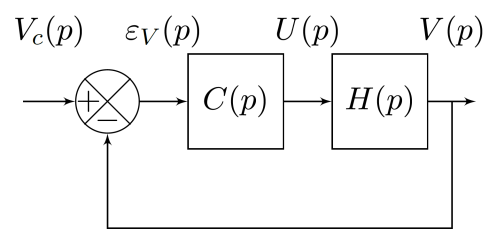
\includegraphics[width=.4\linewidth]{image12}
\caption{\label{fig:CCMP:2021:12} Schéma-blocs simplifié (sans perturbation)}
\end{figure}  

$H(p)=\dfrac{K_N}{\left(1+T_m p\right) \left(1+T_e p\right)}$. 
Avec : $K_N=\SI{20}{m.s^{-1}.V^{-1}}$ avec $T_m\simeq \SI{5}{s}$	$T_e\simeq\SI{0,5}{s}$.
 

Le concepteur a choisi un correcteur Proportionnel Intégral :	$C_1 (p)=\dfrac{C}{T_i p} \left(1+T_i p\right)$ avec $T_i=T_m$.

% Q26
\question{\label{q:CCMP:2021:26}Déterminer les expressions littérales de l'erreur statique $E_S$ (consigne : échelon d'amplitude $V_0$) et de l'erreur de trainage $E_T$ (consigne : rampe de pente $\gamma_0$) de cet asservissement corrigé avec $C_1 (p)$ en fonction de la consigne, du gain $K_N$ et des paramètres du correcteur $C$ et $T_m$. En déduire la condition (notée $C_{\varepsilon}$) sur le gain $C$ du correcteur permettant de satisfaire l’exigence 1.2.3 du cahier des charges.}
\ifprof
\begin{corrige}
\textbf{Méthode recommandée -- Classe de la BO}

La FTBO peut s'exprimer sous la forme $F(p)=\dfrac{C}{T_i p} \left(1+T_i p\right)\dfrac{K_N}{\left(1+T_m p\right) \left(1+T_e p\right)}$ $=\dfrac{C}{T_m p}\dfrac{K_N}{ \left(1+T_e p\right)}$. $F(p)$ est une fonction de classe 1 et de gain $\indice{K}{BO} = \dfrac{CK_N}{T_m} $.

L'erreur statique $E_S$ est alors nulle. L'erreur de trainage $E_t$ est donnée par  $E_t = \dfrac{\gamma_0 T_m}{C K_N}$ $ =\dfrac{1,6\times 5}{C \times 20}$. Pour valider l'exigence, il faut donc $\dfrac{0,4}{C} \leq 0,16 $
$\Rightarrow C\geq  \SI{2,5}{sVm^{-1}}$.

\begin{center}
\begin{tabular}{p{5cm}llp{3cm}}
\hline
Exigence & Cahier des charges & Calcul & Validation  \\
\hline
Erreur statique pour une entrée $V_0 = \SI{8}{m.s^{-1}}$ & $E_S=0$ & $E_S=0$ & Validé \\
Erreur de trainage pour une entrée $\gamma_0 = \SI{1,8}{m.s^{-2}}$ & $E_T\leq \SI{0,16}{m.s^{-1}}$ &  & Validé pour  $C\geq  \SI{2,5}{sVm^{-1}}$\\
\hline
\end{tabular}
\end{center} 
\end{corrige}
\else
\fi

Les diagrammes de Bode de la fonction de transfert en boucle ouverte corrigée de l'asservissement avec $C_1 (p)$ sont fournis sur le cahier réponse à la question \ref{q:CCMP:2021:27} (il sont aussi donnés Figure \ref{fig:CCMP:2021:bode}). Ces diagrammes de Bode ont été tracés avec la valeur particulière $C=1$.


\begin{figure}[!h]
\centering
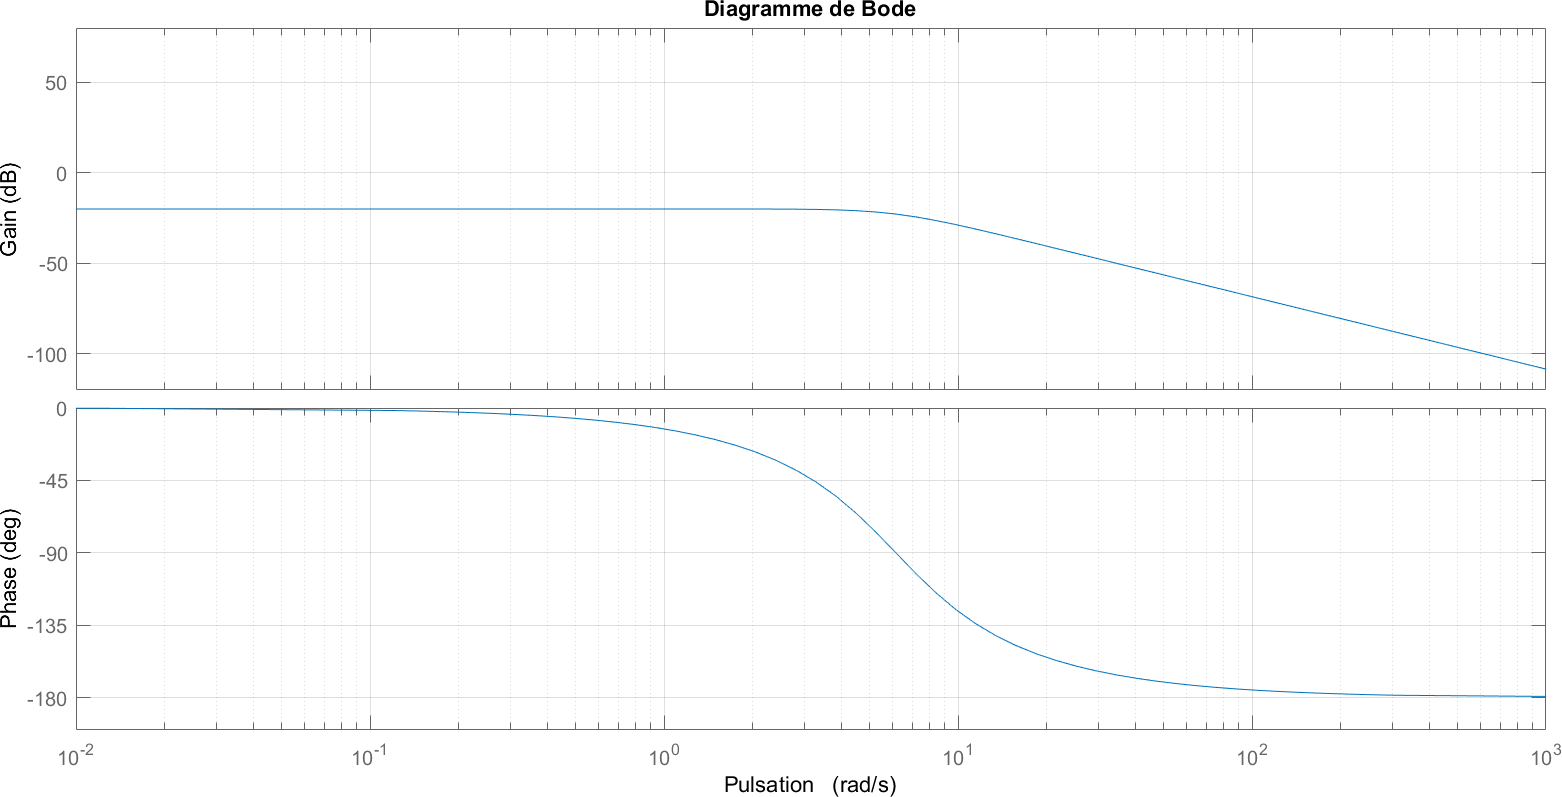
\includegraphics[width=.45\linewidth]{Bode}
\caption{\label{fig:CCMP:2021:bode} Réponse à un échelon d’amplitude $V_0=\SI{8}{m.s^{-1}}$.}
\end{figure} 

% Q27
\question{\label{q:CCMP:2021:27}Déterminer la condition (notée $C_{\varphi}$) sur le gain $C$ du correcteur permettant de satisfaire uniquement le critère de marge de phase de l’exigence 1.2.2 du cahier des charges. Faire l’application numérique (on pourra utiliser la courbe fournie en annexe 1).}
\ifprof
\begin{corrige}
D'après le cahier des charges, on souhaute une marge de phase supérieure à 45\degres.
Cette marge est obtenue pour une pulsation de \SI{2}{rad.s^{-1}}. À cette pulsation, le gain de la BO non corrigée est de \SI{2,5}{dB}. 

On cherche donc $C_\varphi$ tel que $20\log C_\varphi = -2,5$ $\Rightarrow C_\varphi = 10^{-2,5/20} = 0,75$.
Il faut donc que $C_\varphi$ soit inférieur à \SI{0,75}{mVs^{-1}} pour que la marge de phase soit supérieure à 45\degres.
\end{corrige}
\else
\fi

% Q28
\question{\label{q:CCMP:2021:28}Conclure quant à la capacité de ce correcteur à satisfaire le cahier des charges.}
\ifprof
\begin{corrige}
On a vu que :
\begin{itemize}
\item $C\geq  \SI{2,5}{sVm^{-1}}$;
\item $C_{\varphi} \leq  \SI{0,75}{mVs^{-1}}$.
\end{itemize}

Il n'est donc pas possible de satisfaire le cahier des charges avec un correcteur proportionnel. 

\end{corrige}
\else
\fi

\subsection{Réglage du correcteur PID}
On choisit finalement de prendre le correcteur Proportionnel Intégral Dérivé suivant :
$C_2 (p)=C \left(1+\dfrac{1}{T_i p}+T_d p\right)$ avec $T_i=2 T_e$  et $T_d=\dfrac{T_e}{2}$.

% Q29
\question{\label{q:CCMP:2021:29}Montrer qu'on peut mettre ce correcteur sous la forme $C_2 (p)=\dfrac{K}{p} \left(1+T p\right)^2$ et donner les expressions de $K$ et de $T$ en fonction de $C$ et $T_e$.}
\ifprof
\begin{corrige}
On a d'une part, $C_2 (p)=C \left(1+\dfrac{1}{2 T_e p}+\dfrac{T_e}{2} p\right)$ $=\dfrac{C}{2 T_e }\dfrac{1 +2 T_e p +  T_e^2p^2}{p}$.

D'autre part $C_2 (p)=\dfrac{K}{p} \left(1+2 TP+ T^2 p^2\right)$.

En identifiant, $T=T_e$ et $K = \dfrac{C}{2 T_e }$.
\end{corrige}
\else
\fi

% Q30
\question{\label{q:CCMP:2021:30}Donner l'expression de la fonction de transfert en boucle ouverte du système corrigé. En déduire les expressions littérales de l'erreur statique $E_S$ (consigne : échelon d'amplitude $V_0$) et de l'erreur de trainage $E_T$ (consigne : rampe de pente $\gamma_0$) de cet asservissement corrigé. En déduire la condition sur la valeur du gain $K$ du correcteur permettant de satisfaire l’exigence 1.2.3 du cahier des charges.}
\ifprof
\begin{corrige}
La FTBO du système corrigé est donnée par $F_2(p)=\dfrac{K}{p} \left(1+T p\right)^2\dfrac{K_N}{\left(1+T_m p\right) \left(1+T_e p\right)}$.

Cette fonction étant de classe 1 et de gain $KK_N$, on a $E_S = 0$ et $E_T = \dfrac{\gamma_0}{KK_N}$. Pour respecter l'exigence 1.2.3, il faut donc nécessaurement que $\dfrac{\gamma_0}{KK_N} \leq 0,16$ soit 
$\dfrac{\gamma_0}{0,16K_N} \leq K$. On a donc $K\geq \dfrac{1,6}{0,16\times 20}$ $=\SI{0,5}{V m^{-1}}$.
\end{corrige}
\else
\fi


% Q31
\question{\label{q:CCMP:2021:31}La courbe réelle de la phase de la FTBO est représentée sur le cahier réponses et Figure \ref{fig:CCMP:2021:bode2}. Compléter le tracé avec les diagrammes de Bode asymptotiques (gain et phase) de la FTBO du système corrigé avec le correcteur $C_2 (p$) (avec $K=\SI{0,05}{V.m^{-1}}$). On assimilera la courbe réelle de gain à son tracé asymptotique. Tracer la marge de phase sur le cahier réponses et conclure quant au respect du cahier des charges.}
\ifprof
\begin{corrige}
\end{corrige}
\else
\fi

\begin{figure}[!h]
\centering
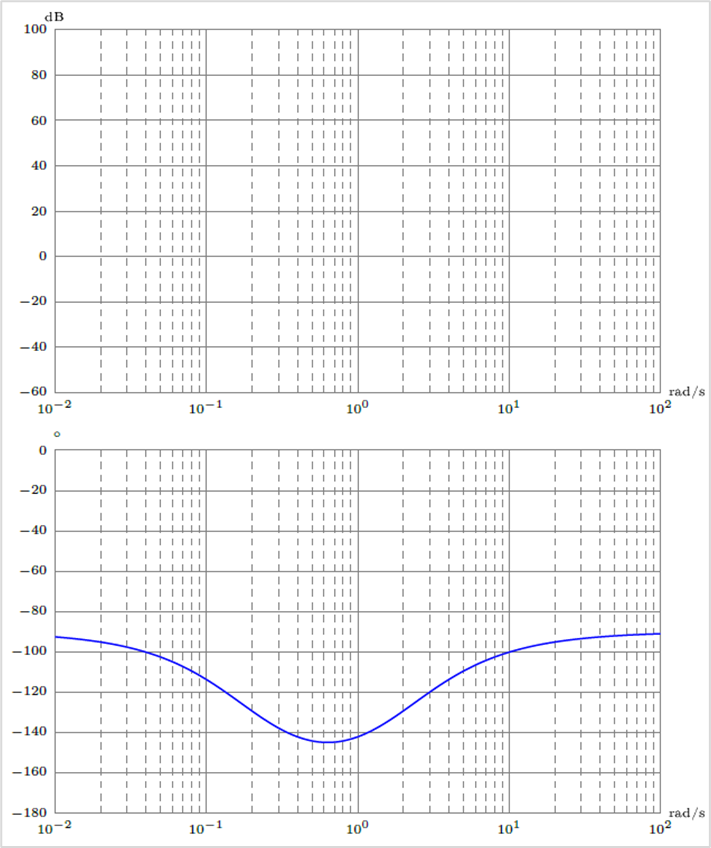
\includegraphics[width=.45\linewidth]{Bode2}
\caption{\label{fig:CCMP:2021:bode2}}
\end{figure} 


On choisit finalement le réglage du correcteur $C_2 (p)$ suivant, qui permet de satisfaire l’exigence 1.2.2 :
$C_2 (p)=\dfrac{7,5}{p} (1+0,5 p)^2$
On réalise une simulation, dont les résultats sont donnés sur la Figure \ref{fig:CCMP:2021:13}, la Figure \ref{fig:CCMP:2021:14} et la Figure \ref{fig:CCMP:2021:15}. 

% Q32
\question{\label{q:CCMP:2021:32}Relever la valeur du premier dépassement puis du temps de réponse pour le système soumis à un échelon. Relever le dépassement pour le système soumis à un trapèze de vitesse. Conclure quant à la capacité de ce correcteur à satisfaire l’exigence 1.2 du cahier des charges.}
\ifprof
\begin{corrige}
Le pic est atteint à \SI{8,7}{m.s^{-1}}. Le dépassement absolu est donc de \SI{0,7}{m.s^{-1}} et le dépassement relatif est donc de 8\,\%. Cela est bien inférieur aux 10\,\% exigés par le cahier des charges. 

Pour la réponse à un trapèze le dépassement relatif est inférieur à $\SI{0,1}{m.s^{-1}}$.


\textbf{Bilan :}
\begin{center}
\begin{tabular}{p{5cm}llp{3cm}}
\hline
Exigence & Cahier des charges & Mesure& Validation  \\
\hline
Rapidité & $T_{5\%}\leq \SI{3}{s}$ & & \\
Stabilité & $M_G\geq\SI{12}{dB}$ & & \\
	& $M_{\varphi} \geq\SI{45}{\degres}$ & & \\
Erreur statique pour une entrée $V_0 = \SI{8}{m.s^{-1}}$ & $E_S=0$ & $E_S=0$ & Validé \\
Erreur de trainage pour une entrée $\gamma_0 = \SI{1,8}{m.s^{-2}}$ & $E_T\leq \SI{0,16}{m.s^{-1}}$ &  & Validé pour  $C\geq  \SI{2,5}{sVm^{-1}}$\\
Dépassement & $D_{1E} \leq 10\%$ & & \\
		   & $D_{1T} \leq \SI{0,1}{m.s^{-1}}$ & & \\
\hline
\end{tabular}
\end{center} 

\end{corrige}
\else
\fi

\begin{figure}[!h]
\centering
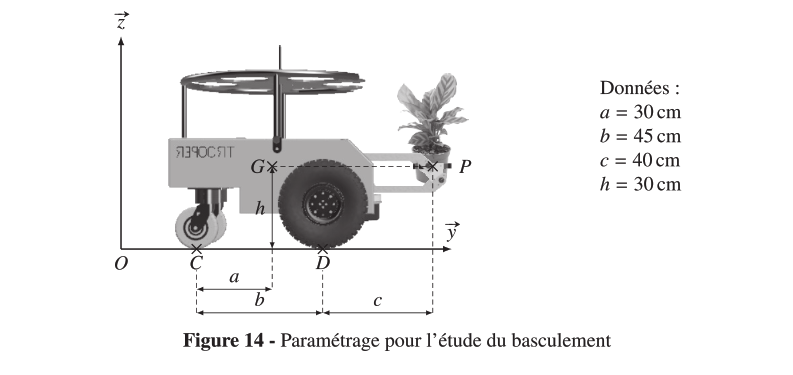
\includegraphics[width=.45\linewidth]{image13}
\caption{\label{fig:CCMP:2021:13} Réponse à un échelon d’amplitude $V_0=\SI{8}{m.s^{-1}}$.}
\end{figure} 
 
\begin{figure}[!h]
\centering
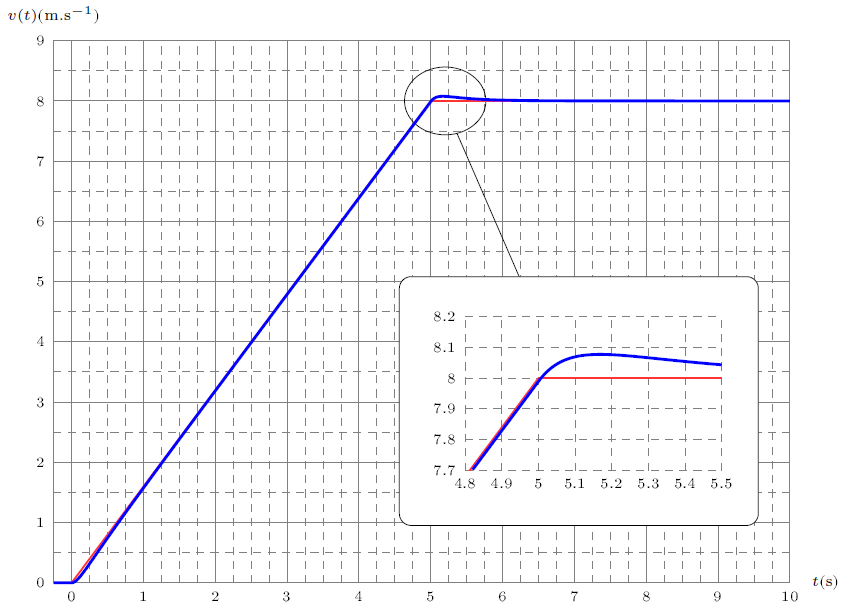
\includegraphics[width=.45\linewidth]{image14}
\caption{\label{fig:CCMP:2021:14} Réponse à un trapèze de vitesse avec $V_0=\SI{8}{m.s^{-1}}$ et accélération maximale $\gamma_0$}
\end{figure} 

\begin{figure}[!h]
\centering

\includegraphics[width=.45\linewidth]{image15}
\caption{\label{fig:CCMP:2021:15} Evolution de la tension moteur soumis à une consigne en trapèze de vitesse.}
\end{figure} 


% Q33
\question{\label{q:CCMP:2021:33}Commenter la courbe de tension du moteur (Figure \ref{fig:CCMP:2021:15}) pour une consigne en trapèze de vitesse. Au vu de cette analyse, proposer une modification du modèle de la Figure \ref{fig:CCMP:2021:10} afin de limiter les écarts entre la simulation et le comportement réel du système.}
\ifprof
\begin{corrige}
\end{corrige}
\else
\fi

